\documentclass[10pt, a4paper]{article}
\usepackage{lrec2016}
\usepackage{multibib}
\newcites{languageresource}{Language Resources}
\usepackage{graphicx}
% for eps graphics

\usepackage{epstopdf}
\usepackage[latin1]{inputenc}
 

\title{Open Source Code Serving Endangered Languages}

\name{Richard Littauer}

\address{Saarland University\\ %, Affiliation2, Affiliation3 \\
         Saarbr\"ucken, Germany\\%, Address2, Address3 \\
         richard.littauer@gmail.com\\}%, author2@zzz.edu, author3@hhh.com\\}


\abstract{
We present a database of open source code that can be used by low-resource language
communities to build digital resources. Our database is also useful to software developers
working with those communities and to researchers looking to describe the state of the field
when seeking funding for development projects.  \\ 
\newline 
\Keywords{open source, under resourced languages, ontology, database, endangered languages, code} }

\begin{document}

\maketitleabstract

\section{Introduction}

Almost half of the approximately 7,000 currently spoken languages are expected to
become extinct this century; it is estimated that less than 5\% of these will be used online or have
significant digital presence \cite{kornai2013digital}. Languages which do not have significant digital
resources (often called low-resource, under-resourced, or minority languages) risk extinction
from loss of prestige, specific domain usage (such as online), and ultimately loss of speakers.
Many language communities and academics working with them try to prevent this by developing
tools, websites, and resources for their languages. However, these approaches are fragmented,
often incurring large developmental and funding costs for single, non-extensible use cases.

To make this process easier for all stakeholders, we have built the first database (to our knowledge)
of all open source code projects related to low-resource languages.

Our database is structured as a simple list in Markdown format, hosted in a GitHub
repository. GitHub is the largest online network of open source code and allows for parallel
collaborative development, while providing critical collaborating support via a built in wiki,
issue tracking and comments on new suggestions. The features provided by Github are
increasingly important to academics and the field of education (Zagalsky 2015). These features
were not available via previous code and text sharing solutions such as SourceForge and are
often not available via institutional repositories. Our list is structurally simple, shareable, easily
updated, and part of a wider cultural movement on GitHub of using Markdown files as simple
databases (Sorhus 2013). Our list monopolizes on the low barrier of entry on GitHub (Storey et
al. 2014). Our list currently describes over 241 open source projects, which includes specific
sections for extensible code for over 26 different languages.

Our solution is open source, not just in the sense of code and data availability (or disclosure) but
in the sense of collaborative involvement and inclusive discussion. By using a solution like
GitHub we were able to reach out to both developers and researchers. Our list is updatable more
rapidly than previous solutions like http://lingtransoft.info/. We mitigate the risk of a single point
of failure (a recent issue with LinguistList) by working in a distributed fashion. The data in our
list is open and can be copied and reused by anyone, something not necessarily true of previous
solutions. By choosing a commercial solution, we sidestep many of the institution issues
associated with archives and repositories currently servicing academics.

Our ultimate goal is a collaboratively built and maintained resource for highlighting
useful, extensible code for low-resource languages. We would like to share our current efforts
and welcome communication with the wider academic linguistics community.

TODO Answer this better
% Questions to answer:
% How is this an innovative way to provide resources, and how is it an innovative way of collecting existing methods?

\section{Database structure}
TODO Fill this out
% Questions to answer:
% Can I have an example? And a basic description of the projects structure?

\subsection{Overall structure}
TODO Fill this out

\subsection{Example entry}
TODO Fill this out

\section{Personas}
TODO Fill this out
% Questions to answer:
% It is clear that this project is intended at linguists. Would good to develop or pitch in such a way that it can be useful to community members (who may not have the resource of a linguist)?

\section{Commitments}

TODO Fill this out
% Questions to answer:
% What are the stakeholders' commitments to this project? Bearing in mind that it serves under-resourced communities that will always exist, it will be good to hear how such a project may exist for a good duration.
% Because this is open-source, are there guidelines in place for the misuse of available code and projects?
% Is there a central community that will be able to advise users who face difficulties when using the system?

\section{Conclusion}

TODO: Add the references in 
%% References
%-1. Endangered Languages. https://www.github.com/RichardLitt/endangered-languages
%-2 Kornai A (2013) Digital Language Death. PLoS ONE 8(10): e77056. doi:10.1371/journal.pone.0077056
%-3 GitHub. https://www.github.com
%-4 SourceForge. https://www.sourceforge.com
%-5 Sindre Sorhus?s list of awesome-lists. https://github.com/sindresorhus/awesome
%6. Lingtransoft. http://lingtransoft.info/
%7. Linguist List. 


% Past reviewer statements

% Reviewer 1:
% The abstract states the problem well - namely, that languages with few resources need more computational support.

% The main point seems to be that the author has collected a list of other people's work. However, I find it impossible to determine whether the author's work supports the main point due to the lack of examples or even a basic description of the project's structure. It does not seem innovative in that it does not seek to present a new method for providing resources, only a new way of collecting existing methods.

% If the work is as described, it is relevant to the field and may have a significant impact on applied linguistic material & resource creation for less-served language communities. It's just very difficult to assess it without sufficient evidence.
% Reviewer 2:

% The authors present an interesting project, well suited for a poster or digital poster presentation, but not for an oral presentation.
% Many participants at the LSA would benefit from learning about this project and vice versa the authors would find additional resources among the participants.
% Reviewer 3:

% This is a presentation of a tool rather than a research paper. Maybe include results from testing for particular languages.
% Reviewer 4:

% This paper is valuable as it mitigates a basic problem in the field of language documentation, extending a potential wealth of resources to those who would traditionally have higher barriers to them.

% There are a few basic questions that ought to be addressed: 

% It is clear that this project is intended at linguists. Would good to develop or pitch in such a way that it can be useful to community members (who may not have the resource of a linguist)?

% What are the stakeholders' commitments to this project? Bearing in mind that it serves under-resourced communities that will always exist, it will be good to hear how such a project may exist for a good duration.

% Because this is open-source, are there guidelines in place for the misuse of available code and projects?

% Is there a central community that will be able to advise users who face difficulties when using the system?

% I would recommend this as a paper rather than a poster, seeing that this brings valuable a new valuable tool to the field. It might not be as effective in poster form.


%
%\section{Citing References in the Text}
%
%\subsection{Bibliographical References}
%
%All bibliographical references within the text should be placed in parentheses
%containing the author's surname followed by a comma before the date of
%publication \cite{Martin-90}. If the sentence already includes the author's
%name, then it is only necessary to put the date in parentheses:
%\newcite{Martin-90}. When several authors are cited, those references should be
%separated with a semicolon: \cite{Martin-90,CastorPollux-92}. When the reference
%has more than three authors, only cite the name of the first author followed by
%et al. (e.g. \cite{Superman-Batman-Catwoman-Spiderman-00}).
%%
%\subsection{Language Resource References}
%
%\subsubsection{When Citing Language Resources}
%
%When mentioning language resources, we recommend that they are cited in
%a similar way to bibliographical references, except that, in order to make them
%appear in a separate section, you need to use the
%\texttt{\\citelanguageresource} tag. Thus, a language resource should be cited
%as \citelanguageresource{speecon}.
%
%
%\subsubsection{When Not Citing Any Language Resource}
%
%When no language resource needs to be cited in the paper, you need to comment
%out a few lines in the \texttt{.tex} file:
%
%\begin{verbatim}
%% \usepackage{multibib}
%% \newcites{languageresource}{}
%% \section{Language Resource References}
%% \bibliographystylelanguageresource
%%   {lrec2016}
%% \bibliographylanguageresource{xample}
%\end{verbatim}
%
%\section{Figures \& Tables}
%\subsection{Figures}
%
%All figures should be centred and clearly distinguishable. They should never be
%drawn by hand, and the lines must be very dark in order to ensure a high-quality
%printed version. Figures should be numbered in the text, and have a caption in
%Times 10 pt underneath. A space must be left between each figure and its
%respective caption. 
%
%Example of a figure enclosed in a box:
%
%\begin{figure}[!h]
%\begin{center}
%%\fbox{\parbox{6cm}{
%%This is a figure with a caption.}}
%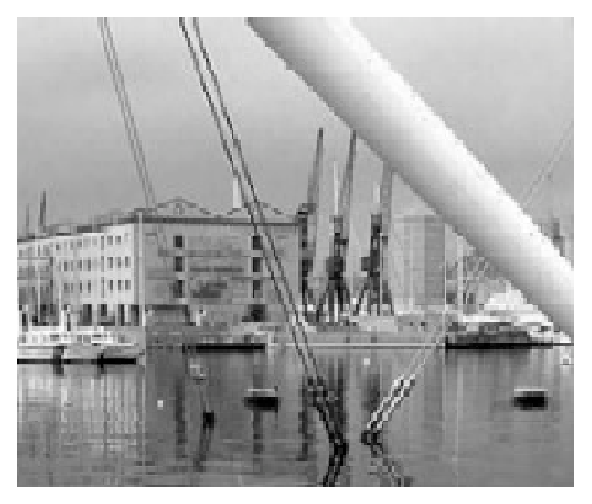
\includegraphics[scale=0.5]{image1.eps} 
%\caption{The caption of the figure.}
%\label{fig.1}
%\end{center}
%\end{figure}
%
%Figure and caption should always appear together on the same page. Large figures
%can be centred, using a full page.
%%NB: an example of large figures is missing.  \newpage
%
%\subsection{Tables}
%
%The instructions for tables are the same as for figures.
%%Two types of tables are distinguished: in-column and big tables that don't fit in the columns.
%%\subsection{In-column tables}
%%An example of an in-column table is presented here.
%%
%\begin{table}[!h]
%\begin{center}
%\begin{tabular}{|l|l|}
%
%      \hline
%      Level&Tools\\
%      \hline\hline
%      Morphology & Pitrat Analyser\\
%      Syntax & LFG Analyser (C-Structure)\\
%     % Semantics & LFG F-Structures + Sowa's\\
%     % & Conceptual Graphs\\
%      \hline
%
%\end{tabular}
%\caption{The caption of the table}
% \end{center}
%\end{table}
%
%%\subsection{Big tables}
%%
%%An example of a big table which extends beyond the column and will
%%float in the next page.
%%
%% \begin{table*}[ht]
%% \begin{center}
%% \begin{tabular}{|l|l|}
%%
%%       \hline
%%       Level&Tools\\
%%       \hline\hline
%%       Morphology & Pitrat Analyser\\
%%       Syntax & LFG Analyser (C-Structure)\\
%%       Semantics & LFG F-Structures + Sowa's Conceptual Graphs  \\
%%       \hline
%%
%% \end{tabular}
%% \caption{The caption of the big table}
%% \end{center}
%% \end{table*}
%%
%
%\section{Footnotes}
%
%Footnotes are indicated within the text by a number in superscript\footnote{They
%should be in Times 9, and appear at the bottom of the same page as their
%corresponding number. Footnotes should also be separated from the rest of the
%text by a horizontal line 5 cm long.}.
%
%\section{Copyrights}
%
%The The Lan\-gua\-ge Re\-sour\-ce and Evalua\-tion Con\-fe\-rence (LREC)
%proceedings are published by the European Language Resources Association (ELRA).
%They are available online from the conference website.
%
%
%ELRA's policy is to acquire copyright for all LREC contributions. In assigning
%your copyright, you are not forfeiting your right to use your contribution
%elsewhere. This you may do without seeking permission and is subject only to
%normal acknowledgement to the LREC proceedings. The LREC 2016 Proceedings are
%licensed under CC-BY-NC, the Creative Commons Attribution-NonCommercial 4.0
%International License.
%
%\section{Conclusion}
%
%Your submission of a finalized contribution for inclusion in the LREC
%proceedings automatically assigns the above-mentioned copyright to ELRA.
%
%
%\section{Acknowledgements}
%
%Place all acknowledgements (including those concerning research grants and
%funding) in a separate section at the end of the article.
%
%\section{Providing References}
%
%\subsection{Bibliographical References}
%Bibliographical references should be listed in alphabetical order at the
%end of the article. The title of the section, ``Bibliographical References'',
%should be a level 1 heading. The first line of each bibliographical reference
%should be justified to the left of the column, and the rest of the entry should
%be indented by 0.35 cm.
%
%The examples provided in Section \ref{main:ref} (some of which are fictitious
%references) illustrate the basic format required for articles in conference
%proceedings, books, journals articles, Ph.D. theses, and chapters of books.
%
%\subsection{Language Resource References}
%
%Language resource references should be listed in alphabetical order at the end
%of the article, in the ``Language Resource References'' section, placed after
%the ``Bibliographical References'' section. The title of the ``Language Resource
%References'' section, should be a level 1 heading. The first line of each
%language resource reference should be justified to the left of the column, and
%the rest of the entry should be indented by 0.35 cm. The example in Section 
%\ref{lr:ref} illustrates the basic format required for language resources.
%
%In order to be able to cite a language resource, it must be added to
%the \texttt{.bib} file first, as a \texttt{@LanguageResource} item type, which
%contains the following fields:
%
%\begin{itemize}
%    \item{\texttt{author}: the builder of the resource}
%    \item{\texttt{title}: the name of the resource}
%    \item{\texttt{publisher}: the publisher of the resource (project,
%          organization etc)}
%    \item{\texttt{year}: year of the resource release}
%    \item{\texttt{series}: more general resource set this language resource
%          belongs to}
%    \item{\texttt{edition}: version of the resource}
%    \item{\texttt{islrn}: the International Standard Language Resource Number
%          (ISLRN) of the resource\footnote{The ISLRN number is available from
%          \texttt{http://islrn.org}}} 
%\end{itemize}
%
%If you want the full resource author name to appear in the citation, the
%language resource author name should be protected by enclosing it between
%\texttt{\{...\}}, as shown in the model \texttt{.bib} file.
%
%\section*{Appendix: How to Produce the \texttt{.pdf} Version}
%
%In order to generate a PDF file out of the LaTeX file herein, when citing
%language resources, the following steps need to be performed:
%
%\begin{itemize}
%    \item{Compile the \texttt{.tex} file once}
%    \item{Invoke \texttt{bibtex} on the eponymous \texttt{.aux} file}
%    \item{Invoke \texttt{bibtex} on the \texttt{languageresources.aux} file}
%    \item{Compile the \texttt{.tex} file twice}
%\end{itemize}

% \nocite{*}
\section{Bibliographical References}
\label{main:ref}

\bibliographystyle{lrec2016}
\bibliography{xample}


\section{Language Resource References}
\label{lr:ref}
\bibliographystylelanguageresource{lrec2016}
\bibliographylanguageresource{xample}

\end{document}
